\documentclass[tikz,border=2pt]{standalone}
\usepackage{pgfplots}
\usetikzlibrary{intersections,calc,matrix,arrows,decorations.pathmorphing}
\usepgfplotslibrary{fillbetween}
\pgfplotsset{compat=1.7}

\tikzset{
  declare function={
  	EDPVR(\x, \C)= -0.4 - (\C/-0.0346)*(1 - e^(+0.0345*\x));
  	}
}



\begin{document}
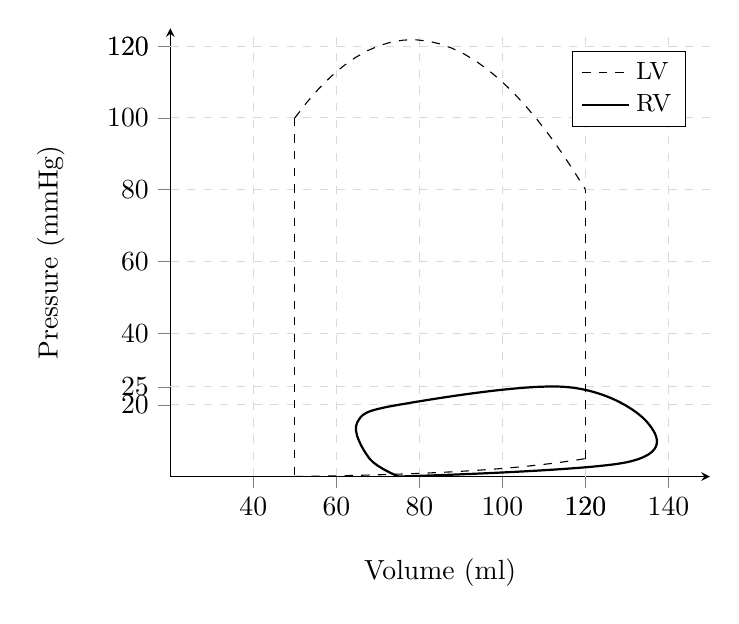
\begin{tikzpicture}

\begin{axis}[
        axis lines=middle,
        grid = major,
        grid style={dashed, gray!30},
	ymin = 0,
	ymax = 125,
	xmin = 20,
	xmax =150,
	 ylabel near ticks,
	xlabel near ticks,
	extra y ticks={25, 120},
	extra x ticks={120},
        xlabel=Volume (ml),
        ylabel=Pressure (mmHg),
        tick align=outside,
        enlargelimits=false,
	legend pos= north west,
	legend style={font=\small, cells={align=left}, at={(0.85,0.95)},anchor=north},
	legend cell align={left}]

\node (o) at (axis cs: 0,0){};

\draw[black, thick] plot[smooth,tension=0.6] coordinates { (axis cs: 75,0) (axis cs: 130,4) (axis cs: 135, 15) (axis cs: 115, 25) (axis cs: 75, 20) (axis cs: 65,15) (axis cs: 68, 5) (axis cs: 75,0)};


%normal loop
\addplot[name path=bot, black, thin, dashed, domain=50:120, forget plot] {-0.400992 - (-0.002991122/-0.03458544)*(1 - e^(+0.03458544*x))};
\draw[black,thin, dashed] (axis cs: 120,5) -- (axis cs: 120,80);
\addplot[name path=top, black, thin, dashed, domain=50:120, forget plot] {-60 + 4.938095*x - 0.03714286*x^2 + 0.00004761905*x^3};
\draw[black, thin, dashed] (axis cs: 50,100) -- (axis cs: 50,0);

%legend
\addlegendimage{black, thin, dashed};
\addlegendentry{LV};
\addlegendimage{black, thick};
\addlegendentry{RV};



\end{axis}

\end{tikzpicture} 
\end{document}